\documentclass[a4paper,14pt]{article}
\usepackage{geometry}
\geometry{letterpaper}
\usepackage{graphicx}
\usepackage{amsmath}
\usepackage{calc}
\usepackage{geometry}
 \geometry{
 a4paper,
 total={170mm,257mm},
 left=25mm,
 right=10mm,
 top=20mm,
 bottom=20mm,
 }

\usepackage{amssymb}
\usepackage[export]{adjustbox}

\vtop{%
  \vskip0pt
  \hbox{%
    \includegraphics{figure}%
  }%
}

\newsavebox{\mybox}
\let\oldincludegraphics\includegraphics
\xdef\maxwidth{0.9\textwidth}
\renewcommand{\includegraphics}[2][]{%
  \savebox{\mybox}{%
    \hbox{\oldincludegraphics[#1]{#2}}}%
\ifdim\wd\mybox>\maxwidth
  \oldincludegraphics[width=50,keepaspectratio]{#2}%
\else
  \oldincludegraphics[#1]{#2}%
\fi}


\ifpdf % We're generating a pdf
    \usepackage[pdftex]{color,graphicx}
    \pdfpagewidth=\paperwidth
    \pdfpageheight=\paperheight
    \usepackage{thumbpdf}
    %\pdfcompresslevel=9
\else
    \usepackage[dvips]{graphicx}
\fi

\pagenumbering{gobble}

\begin{document}
    \raisebox{1ex-\height}{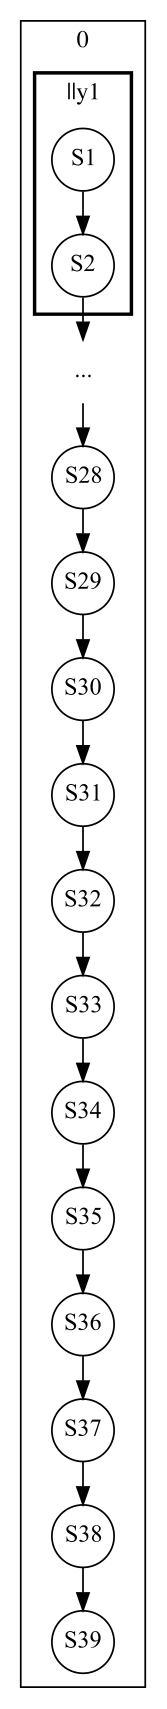
\includegraphics[width=50, height=\textheight,keepaspectratio]{iterations/1.png} }
\raisebox{1ex-\height}{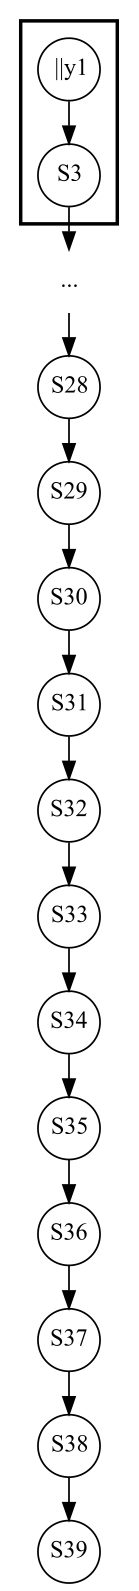
\includegraphics[width=50, height=\textheight,keepaspectratio]{iterations/2.png} }
\raisebox{1ex-\height}{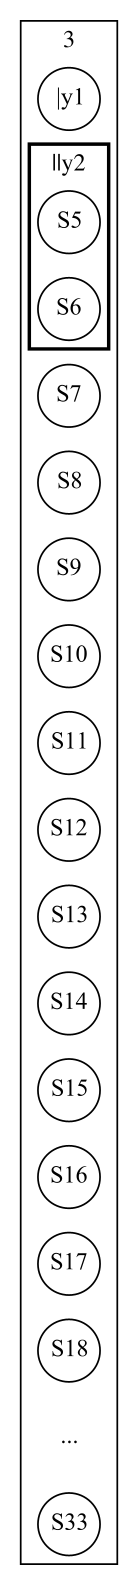
\includegraphics[width=50, height=\textheight,keepaspectratio]{iterations/3.png} }
\raisebox{1ex-\height}{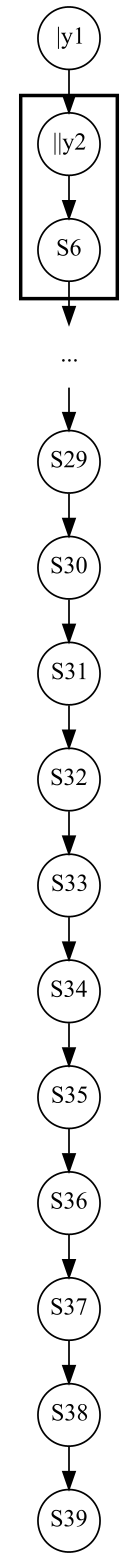
\includegraphics[width=50, height=\textheight,keepaspectratio]{iterations/4.png} }
\raisebox{1ex-\height}{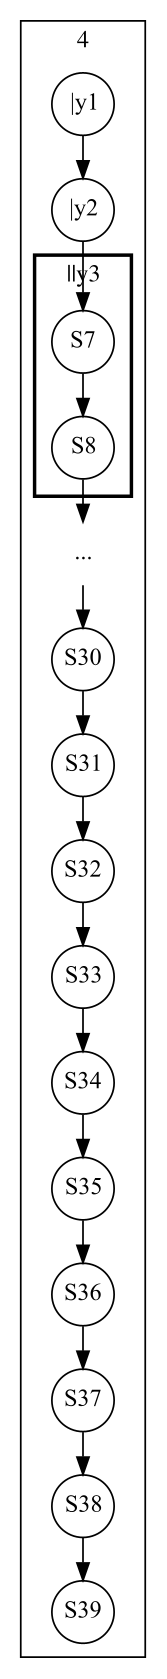
\includegraphics[width=50, height=\textheight,keepaspectratio]{iterations/5.png} }
\raisebox{1ex-\height}{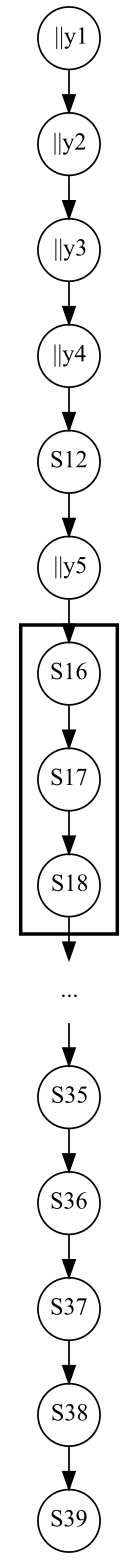
\includegraphics[width=50, height=\textheight,keepaspectratio]{iterations/6.png} }
\raisebox{1ex-\height}{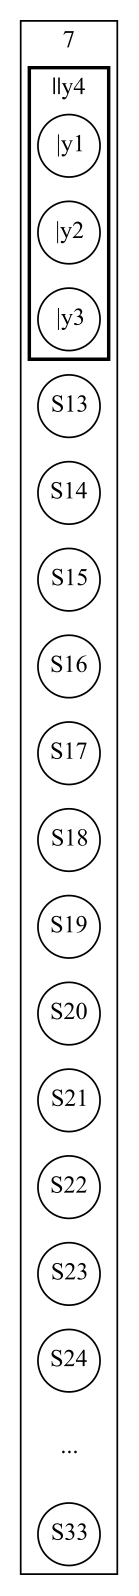
\includegraphics[width=50, height=\textheight,keepaspectratio]{iterations/7.png} }
\raisebox{1ex-\height}{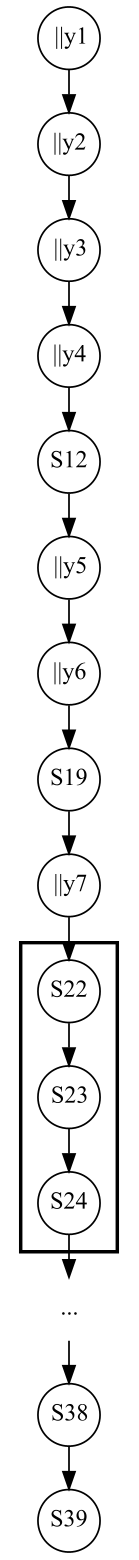
\includegraphics[width=50, height=\textheight,keepaspectratio]{iterations/8.png} }
\raisebox{1ex-\height}{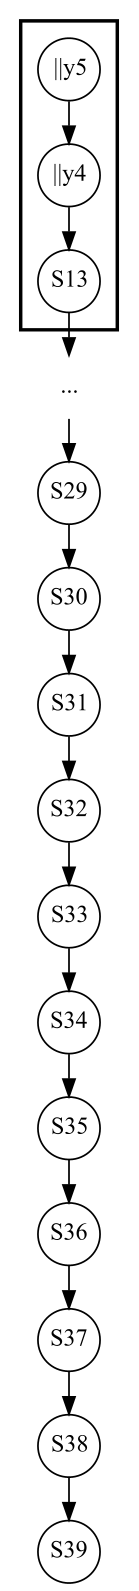
\includegraphics[width=50, height=\textheight,keepaspectratio]{iterations/9.png} }
\raisebox{1ex-\height}{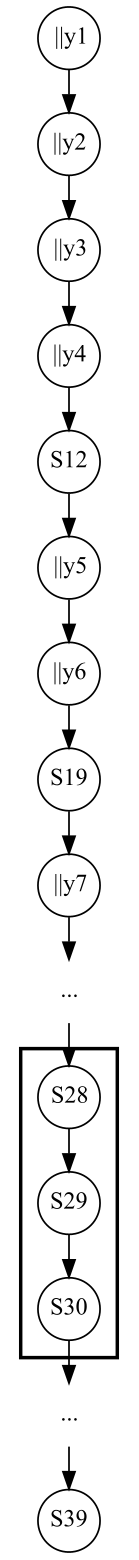
\includegraphics[width=50, height=\textheight,keepaspectratio]{iterations/10.png} }
\raisebox{1ex-\height}{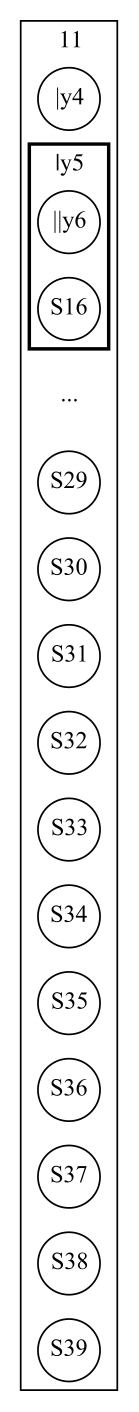
\includegraphics[width=50, height=\textheight,keepaspectratio]{iterations/11.png} }
\raisebox{1ex-\height}{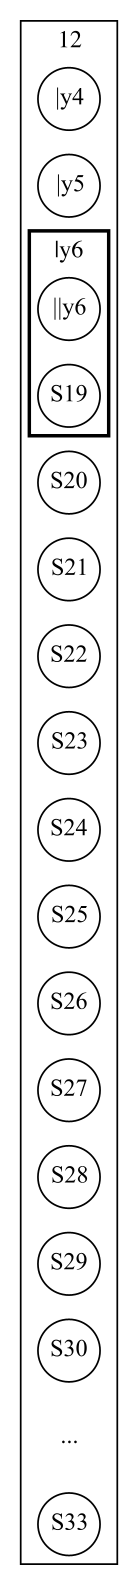
\includegraphics[width=50, height=\textheight,keepaspectratio]{iterations/12.png} }
\raisebox{1ex-\height}{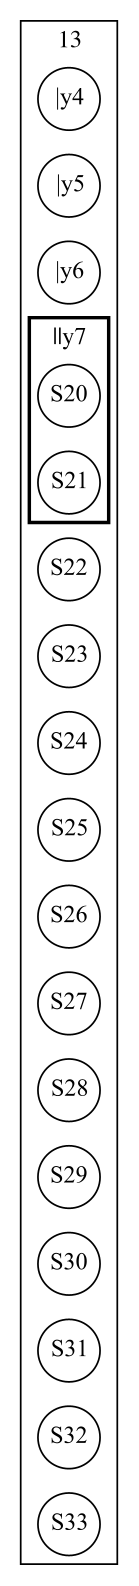
\includegraphics[width=50, height=\textheight,keepaspectratio]{iterations/13.png} }
\raisebox{1ex-\height}{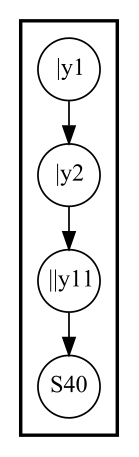
\includegraphics[width=50, height=\textheight,keepaspectratio]{iterations/14.png} }
\raisebox{1ex-\height}{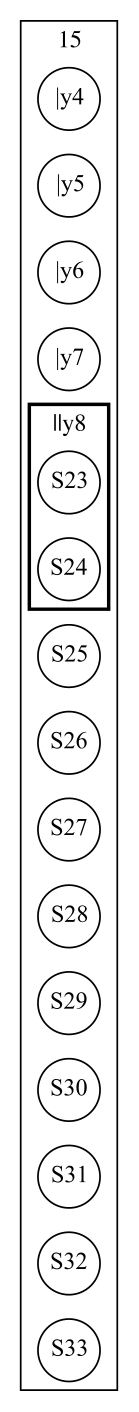
\includegraphics[width=50, height=\textheight,keepaspectratio]{iterations/15.png} }
\end{document}